\chapter{Sensitivity-aware motion planner}
\markboth{Sensitivity-aware motion planner}{}% To set left/right header
% \localtableofcontents

This chapter introduces the first contribution of this thesis, by leveraging the sensitivity concept discussed in Chapter~\ref{chap:models}.
It presents a unified and a decoupled strategies designed to plan trajectories that are both robust and sensitivity-optimal at the same time.
This contribution emphasizes the generation of a desired trajectory with minimal sensitivity, ensuring that the closed-loop evolution of $\q(t)$/$\u(t)$ closely follows its evolution in the nominal case $\q_n(t)$/$\u_n(t)$.
While sensitivity optimization has previously been explored for generating locally sensitivity-optimal trajectories \cite{cPi, cTh}, it has not been applied within a global planning framework that accounts for obstacles.
Furthermore, this contribution introduces the first time the use of the sensitivity-based tubes to enforce constraints in both the state and input spaces.
This enables robust collision checking w.r.t. the environment, but also to check for actuators saturation.

% This chapter first present a unified approach that allow planning a robust trajectory with an optimal sensitivity by directly incorporating the sensitivity computation in an optimal tree building process (e.g. \myglsentry{rrtstar}). 
% The method is applied both on the differential drive robot and the quadrotor, showing some limitations in the latter case.

% Then, the second section present a decoupled approach that shows better efficiency for more complex systems as the quadrotor.

\section{??Sensitivity-aware metrics??}

\subsubsection{Robust collision checking}
The tubes can leverage to perform robust collision check with the environments but also in the control inputs space to avoid actuators saturation. 
Collision checks with the environments are only performed by considering uncertainty in the x y z subspace for simplification.
Several strategies to perform robust collision with the environments:
\begin{enumerate}
    \item One can simply considered a convex bounding shape of the robot and enlarge it by the maximum radius (i.e. the maximum of the worst case deviations). See appendinx for proof.
    \item Compute the bonding box that contains the ellipsoid. Note that even if in this thesis this is the method employed to perform robust collision check, by mean of smooth visualization we depicted the tubes using ellipsoid representation in the various figures.
    \item Compute the ellipsoid semi-axes, and it's orientation w.r.t. the canonical basis of the subspace. However, such orinetation and semi-axis lenght can be obtain by decomposing the kernel into eigenvalues and eigenvectors representation that leads to higher computation times that solely computing the worst deviations. For the quadrotor case, 2000 ellipsoids where computed and the time ratio for the bounding box method over the true ellipsoid computation shows 0.18 times (i.e. bounding box of the true ellipsoid is 5.5 faster to compute instead of true ellipsoid) and the volume shows 172\%, meaning that bounding box faster but a bit conservative as it's approx 1.72 times bigger. Faster because computing the semi axes length requires to pseudo invert K.
\end{enumerate}

\subsubsection{Cost function}

\begin{figure} [t]
    \centering
    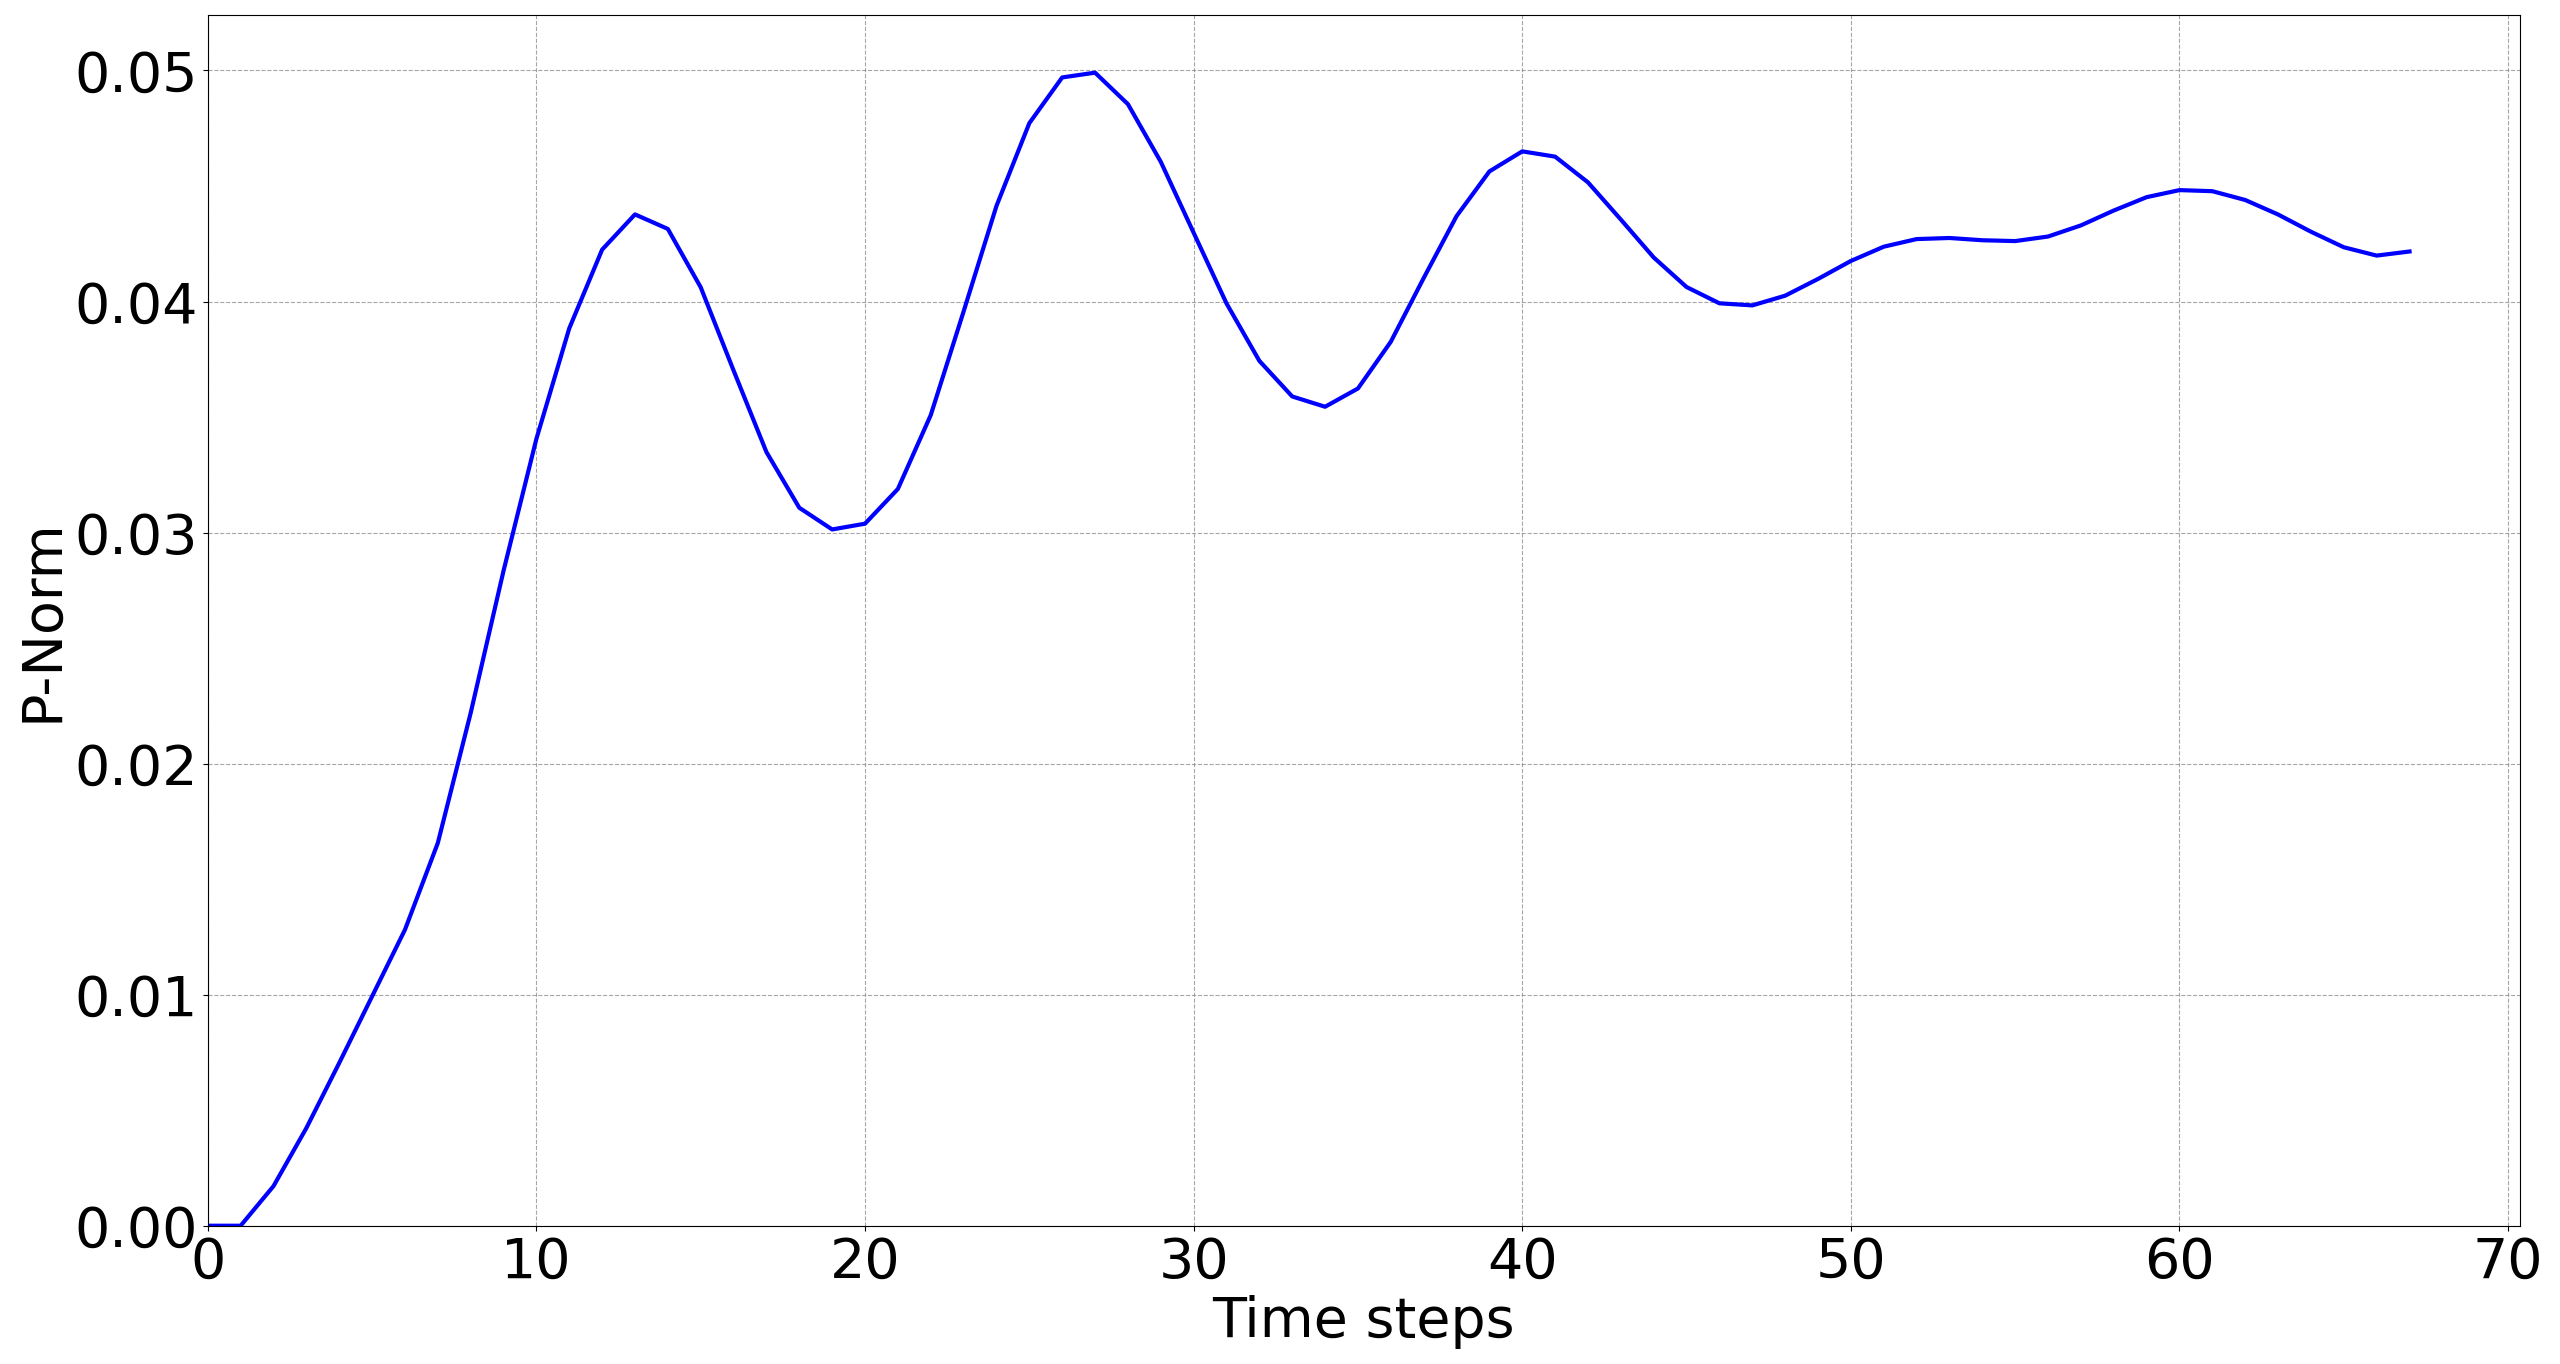
\includegraphics[width=0.8\linewidth]{figures/samp/non_monotoic.png} 
    \caption{Non monotonic p-norm profile along a 70-state trajectory for a quadrotor example.}%
    \label{fig:monotonic}%
\end{figure}

Now that the sensitivity matrices are defined, one can compute and minimize a chosen norm of $\bPi(t)$ and $\bTheta(t)$ w.r.t. the desired trajectory $\q_d(t)$.

However, sensitivity non monotonic and non additive, not suitable for optimal motion planning that requires monotonic and additive cost function properties.
Add figure.

We therefore chose integral.
However, instead of integral of norm of PI as done in~\cite{cPi,cTh}, we chose integral of p-norm radii, better capture deviations to the nominal case.

\section{Unified approach}

This section first present a unified approach that allow planning a robust trajectory with an optimal sensitivity by directly incorporating the sensitivity computation in an optimal planning process (e.g. \myglsentry{rrtstar}).

\subsection{General method}
Explain that ODEs as to be solved each motion check.
Explain roles of init and final conditions, therefore we focus on tree-based approaches.

Remarque complétude.

Additionally, one may compute the ODEs for unbounded local trajectories. 
Leading to high computation times for most of the time unfeasible local trajectories. 
Based on OMPL implementation we chose to use maximum local trajectories length.

\subsection{Algorithms}
\subsubsection{Robust Sensitivity Aware RRT*}
Pseudo code and explain that it is costly because many calls are required to the ODEs (rewiring, optimal connection within radius, etc.).
Explain that the trivial "update children cost" become non trivial as it requires to recimpute the ODEs for eery of them.
\subsubsection{Robust Sensitivity Aware SST*}
Pseudo code and explain that it is more suitable for dynamic propagation as it requires one check per iteration.
Note that in the original version only an open loop approach is considered in the monte carlo propagation, as we are dealing with close loop we rely on a steering method here.

\subsection{Simulation results}
\subsubsection{Differential drive robot}
Results, graph profiling RRT*/RSARRT*, SST*/RSASST*
\subsubsection{Quadrotor robot}
Results, graph profiling RRT*/RSARRT*, SST*/RSASST*

\section{Decoupled approach}
For more complex system such as quadrotor it is still not tracktable. We need to reduce the number of calls again.
\subsection{Algorithms}
\subsubsection{Sensitivity Aware RRT*}
Lazy approach with the tubes, the tree is not robust compared to R-SARRT*, only the final solution is robust.
\subsubsection{Sensitivity Aware Shortcut}
Robust shortcut variant.
Keep the lazy collision check with tubes.

\subsection{Simulation results}
\subsubsection{Differential drive robot}
\subsubsection{Quadrotor robot}

\section{Conclusion}
Approach more efficient when we reduce the number of call. 
However, we still need to improve the computation time.

\todomarker{}